% book_example.tex - Test for Book Class Support (v5.11.x)
% This example tests all book-specific features from v5.11.0 through v5.11.9
% Compiler: LuaLaTeX
%
% Features tested:
%   v5.11.0 - Book class, frontmatter/mainmatter/backmatter, hebrewchapter, hebrewappendix
%   v5.11.1 - 'definition' environment, 'abstract' environment
%   v5.11.2 - TOC BiDi fixes (page numbers LTR, dot leaders)
%   v5.11.3 - \rowcolor{} support in tables
%   v5.11.4 - Code block space artifacts fix
%   v5.11.5 - TOC dot leaders fix
%   v5.11.6 - l@subsubsection TOC formatter
%   v5.11.7-v5.11.9 - TOC RTL alignment fixes

\documentclass[book]{hebrew-academic-template}

\addbibresource{example_references.bib}

\begin{document}

%% ============================================
%% Front Matter
%% ============================================
\frontmatter

%% Title Page
\begin{titlepage}
\begin{center}
\vspace*{2cm}
{\Huge\bfseries ספר בדיקה לתבנית}
\vspace{0.5cm}

{\Large\en{Test Book for Hebrew Academic Template}}
\vspace{1cm}

{\large בדיקת כל תכונות גרסה \en{5.11.x}}
\vspace{2cm}

{\Large מאת}
\vspace{0.5cm}

{\Large\bfseries דר' יורם סגל}
\vspace{3cm}

{\large גרסת \en{CLS}: \clsversion}
\vspace{2cm}

{\normalsize מהדורה ראשונה -- דצמבר \en{2025}}
\end{center}
\end{titlepage}

%% Copyright Page
\newpage
\thispagestyle{empty}
\vspace*{\fill}
\begin{center}
{\small כל הזכויות שמורות \textenglish{©} \en{2025}}
\end{center}
\vspace*{\fill}

%% Abstract (v5.11.1 - New 'abstract' environment for book mode)
\newpage
\begin{abstract}
ספר זה מהווה מדריך מקיף לתבנית האקדמית העברית. התבנית תומכת בכתיבה דו-כיוונית (\en{BiDi}) עבור מסמכים אקדמיים הכוללים עברית ואנגלית.

גרסה \en{5.11} מוסיפה תמיכה מלאה במחלקת ספר (\en{book class}), כולל:
\begin{itemize}
    \item מבנה ספר מלא עם \en{frontmatter/mainmatter/backmatter}
    \item תוכן עניינים, רשימת איורים, ורשימת טבלאות בעברית
    \item פרקים עבריים עם מספור \en{LTR}
    \item נספחים עם מספור עברי (א, ב, ג)
    \item סביבות חדשות כמו \en{definition} ו-\en{abstract}
    \item תמיכה ב-\en{\textbackslash rowcolor\{\}} בטבלאות
\end{itemize}
\end{abstract}

%% Table of Contents
\tableofcontents

%% List of Figures
\listoffigures

%% List of Tables
\listoftables

%% Preface
\chapter*{הקדמה}
\addcontentsline{toc}{chapter}{הקדמה}

זהו ספר בדיקה לבדיקת תמיכת מחלקת הספר (\en{book class}) בתבנית האקדמית העברית גרסאות \en{5.11.0} עד \en{5.11.9}.
התבנית מבוססת על עקרונות מודרניים של עיבוד שפה טבעית \cite{vaswani2017attention}.

\hebrewsection{תכונות \en{v5.11.x} הנבדקות}

\begin{itemize}
    \item \textbf{\en{v5.11.0}}: תמיכת מחלקת ספר (\en{book class})
    \begin{itemize}
        \item \en{frontmatter/mainmatter/backmatter}
        \item \en{\textbackslash hebrewchapter\{\}} ו-\en{\textbackslash hebrewappendix\{\}}
        \item תוכן עניינים, רשימת איורים, רשימת טבלאות בעברית
    \end{itemize}

    \item \textbf{\en{v5.11.1}}: סביבות חדשות
    \begin{itemize}
        \item סביבת \en{abstract} למצב ספר
        \item סביבת \en{definition} לתיבות הגדרה
    \end{itemize}

    \item \textbf{\en{v5.11.2}}: תיקוני \en{TOC BiDi}
    \begin{itemize}
        \item מספרי עמודים ב-\en{LTR}
        \item נקודות מוביל (\en{dot leaders}) תקינות
    \end{itemize}

    \item \textbf{\en{v5.11.3}}: תמיכת צבעי שורות בטבלאות (\en{\textbackslash rowcolor\{\}})

    \item \textbf{\en{v5.11.4}}: תיקון רווחים במחרוזות קוד

    \item \textbf{\en{v5.11.5-v5.11.9}}: תיקוני יישור \en{RTL} בתוכן עניינים
\end{itemize}

\hebrewsection{הפניות לפרקים}

ניתן להפנות לפרקים באמצעות \en{\textbackslash hebrewchapterlabel\{\}} (גרסה \en{5.10.0}):
\begin{itemize}
    \item פרק~\ref{chap:intro} -- פרק ראשון
    \item פרק~\ref{chap:tables} -- טבלאות ואיורים
    \item פרק~\ref{chap:refs} -- הפניות
\end{itemize}

%% ============================================
%% Main Matter
%% ============================================
\mainmatter

%% Chapter 1
\hebrewchapter{פרק ראשון - מבוא}
\hebrewchapterlabel{chap:intro}

זהו הפרק הראשון בספר הבדיקה. המספור צריך להיות \en{1} ב-\en{LTR}.

\hebrewsection{סעיף ראשון}

סעיף זה צריך להיות ממוספר \en{1.1}.

\begin{notebox}[הערה חשובה]
זוהי תיבת הערה (\en{notebox}) עם תמיכת \en{BiDi}. הרקע לא צריך לגלוש מחוץ לשוליים.
\end{notebox}

\hebrewsubsection{תת-סעיף ראשון}

תת-סעיף זה צריך להיות ממוספר \en{1.1.1}.

\begin{examplebox}[דוגמה]
זוהי תיבת דוגמה (\en{examplebox}) עם תמיכת \en{BiDi}.
\end{examplebox}

\hebrewsubsubsection{תת-תת-סעיף}

תת-תת-סעיף זה צריך להיות ממוספר \en{1.1.1.1}.

%% Definition Environment (v5.11.1 - New styled box)
\begin{definition}[הגדרה מתמטית]
\textbf{תבנית אקדמית} היא מסמך \LaTeX{} המותאם לכתיבה אקדמית בעברית ובאנגלית, עם תמיכה מלאה ב-\en{BiDi} (דו-כיווניות).

נוסחה לדוגמה:
\[
E = mc^2
\]

כאשר \en{E} מייצג אנרגיה, \en{m} מסה, ו-\en{c} מהירות האור.
\end{definition}

\hebrewsection{סעיף שני}

סעיף זה צריך להיות ממוספר \en{1.2}.

\begin{warningbox}[אזהרה]
זוהי תיבת אזהרה (\en{warningbox}) עם תמיכת \en{BiDi}.
\end{warningbox}

%% Chapter 2
\hebrewchapter{פרק שני - טבלאות ואיורים}
\hebrewchapterlabel{chap:tables}

פרק זה מדגים טבלאות ואיורים.

\hebrewsection{טבלה לדוגמה}

\begin{hebrewtable}[H]
\caption{טבלת בדיקה}
\label{tab:test}
\begin{rtltabular}{|p{3cm}|p{3cm}|p{3cm}|}
\hline
\textbf{\hebheader{עמודה ג}} & \textbf{\hebheader{עמודה ב}} & \textbf{\hebheader{עמודה א}} \\
\hline
\hebcell{ערך \en{3}} & \hebcell{ערך \en{2}} & \hebcell{ערך \en{1}} \\
\hline
\hebcell{נתון נוסף} & \hebcell{מידע} & \hebcell{תוכן} \\
\hline
\end{rtltabular}
\end{hebrewtable}

%% Row Color Support (v5.11.3 - \rowcolor{} now works in tables)
\hebrewsection{טבלה עם צבעי שורות}

טבלה זו מדגימה את תמיכת \en{\textbackslash rowcolor\{\}} החדשה (גרסה \en{5.11.3}):

\begin{hebrewtable}[H]
\caption{טבלה עם שורות צבעוניות}
\label{tab:colored}
\begin{rtltabular}{|p{3cm}|p{4cm}|p{2cm}|}
\hline
\rowcolor{blue!15}
\textbf{\hebheader{גרסה}} & \textbf{\hebheader{תכונה}} & \textbf{\hebheader{סטטוס}} \\
\hline
\hebcell{\en{v5.11.0}} & \hebcell{תמיכת מחלקת ספר} & \hebcell{פעיל} \\
\hline
\rowcolor{green!10}
\hebcell{\en{v5.11.1}} & \hebcell{סביבות \en{definition} ו-\en{abstract}} & \hebcell{פעיל} \\
\hline
\hebcell{\en{v5.11.3}} & \hebcell{תמיכת \en{\textbackslash rowcolor}} & \hebcell{פעיל} \\
\hline
\rowcolor{yellow!15}
\hebcell{\en{v5.11.9}} & \hebcell{תיקון יישור \en{TOC RTL}} & \hebcell{פעיל} \\
\hline
\end{rtltabular}
\end{hebrewtable}

\hebrewsection{איור לדוגמה}

\begin{figure}[H]
\centering
\begin{english}
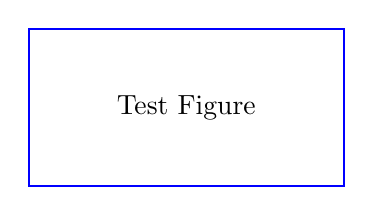
\begin{tikzpicture}
\draw[thick, blue] (0,0) -- (4,0) -- (4,2) -- (0,2) -- cycle;
\node at (2,1) {Test Figure};
\end{tikzpicture}
\end{english}
\caption{איור בדיקה}
\label{fig:test}
\end{figure}

%% Chapter 3
\hebrewchapter{פרק שלישי - הפניות}
\hebrewchapterlabel{chap:refs}

ניתן להפנות לפרק~\ref{chap:intro}, לטבלה~\ref{tab:test}, ולאיור~\ref{fig:test}.

\hebrewsection{קוד לדוגמה}

%% Code Space Artifacts Fix (v5.11.4 - Spaces in strings render correctly)
הקוד הבא מדגים את תיקון רווחי המחרוזות (גרסה \en{5.11.4}). רווחים במחרוזות צריכים להיות נקיים ללא סימנים מיוחדים:

\begin{pythonbox}[\hebtitle{קוד \en{Python} עם רווחים במחרוזות}]
def hello_world():
    # Hebrew comment: פונקציית שלום עולם
    message = "Hello World with spaces"  # Spaces should be clean
    greeting = "שלום עולם"               # Hebrew string
    print(f"Message: {message}")
    print(f"Greeting: {greeting}")
    return True

# Test various string patterns (v5.11.4 fix)
test_strings = [
    "hello world",      # Simple spaces
    "a    b    c",      # Multiple spaces
    "   leading",       # Leading spaces
    "trailing   "       # Trailing spaces
]
\end{pythonbox}

%% ============================================
%% Back Matter
%% ============================================
\backmatter

%% Bibliography
\printbibliography[heading=bibintoc,title={רשימת מקורות}]

%% Appendices
\appendix

\hebrewappendix{נספח ראשון}

זהו הנספח הראשון. המספור צריך להיות א (אלף עברי).

\hebrewappendix{נספח שני}

זהו הנספח השני. המספור צריך להיות ב (בית עברי).

\end{document}
